%%
%% This is file `sample-acmlarge.tex',
%% generated with the docstrip utility.
%%
%% The original source files were:
%%
%% samples.dtx  (with options: `all,journal,bibtex,acmlarge')
%% 
%% IMPORTANT NOTICE:
%% 
%% For the copyright see the source file.
%% 
%% Any modified versions of this file must be renamed
%% with new filenames distinct from sample-acmlarge.tex.
%% 
%% For distribution of the original source see the terms
%% for copying and modification in the file samples.dtx.
%% 
%% This generated file may be distributed as long as the
%% original source files, as listed above, are part of the
%% same distribution. (The sources need not necessarily be
%% in the same archive or directory.)
%%
%%
%% Commands for TeXCount
%TC:macro \cite [option:text,text]
%TC:macro \citep [option:text,text]
%TC:macro \citet [option:text,text]
%TC:envir table 0 1
%TC:envir table* 0 1
%TC:envir tabular [ignore] word
%TC:envir displaymath 0 word
%TC:envir math 0 word
%TC:envir comment 0 0
%%
%% The first command in your LaTeX source must be the \documentclass
%% command.
%%
%% For submission and review of your manuscript please change the
%% command to \documentclass[manuscript, screen, review]{acmart}.
%%
%% When submitting camera ready or to TAPS, please change the command
%% to \documentclass[sigconf]{acmart} or whichever template is required
%% for your publication.
%%
%%
\documentclass[acmlarge]{acmart}
%%
%% \BibTeX command to typeset BibTeX logo in the docs
\AtBeginDocument{%
  \providecommand\BibTeX{{%
    Bib\TeX}}}

%% Rights management information.  This information is sent to you
%% when you complete the rights form.  These commands have SAMPLE
%% values in them; it is your responsibility as an author to replace
%% the commands and values with those provided to you when you
%% complete the rights form.
\setcopyright{acmlicensed}
\copyrightyear{2026}
\acmYear{2026}
\acmDOI{XXXXXXX.XXXXXXX}

%%
%% These commands are for a JOURNAL article.
\acmJournal{AILET}
\acmVolume{01}
\acmNumber{01}
\acmArticle{01}
\acmMonth{01}

%%
%% Submission ID.
%% Use this when submitting an article to a sponsored event. You'll
%% receive a unique submission ID from the organizers
%% of the event, and this ID should be used as the parameter to this command.
%%\acmSubmissionID{123-A56-BU3}

%%
%% For managing citations, it is recommended to use bibliography
%% files in BibTeX format.
%%
%% You can then either use BibTeX with the ACM-Reference-Format style,
%% or BibLaTeX with the acmnumeric or acmauthoryear sytles, that include
%% support for advanced citation of software artefact from the
%% biblatex-software package, also separately available on CTAN.
%%
%% Look at the sample-*-biblatex.tex files for templates showcasing
%% the biblatex styles.
%%

%%
%% The majority of ACM publications use numbered citations and
%% references.  The command \citestyle{authoryear} switches to the
%% "author year" style.
%%
%% If you are preparing content for an event
%% sponsored by ACM SIGGRAPH, you must use the "author year" style of
%% citations and references.
%% Uncommenting
%% the next command will enable that style.
%%\citestyle{acmauthoryear}

\usepackage{listings}

\colorlet{punct}{red!60!black}
\definecolor{background}{HTML}{EEEEEE}
\definecolor{delim}{RGB}{20,105,176}
\colorlet{numb}{magenta!60!black}

\lstdefinelanguage{json}{
    basicstyle=\normalfont\ttfamily,
    numbers=left,
    numberstyle=\scriptsize,
    stepnumber=1,
    numbersep=8pt,
    showstringspaces=false,
    breaklines=true,
    frame=lines,
    backgroundcolor=\color{background},
    literate=
     *{0}{{{\color{numb}0}}}{1}
      {1}{{{\color{numb}1}}}{1}
      {2}{{{\color{numb}2}}}{1}
      {3}{{{\color{numb}3}}}{1}
      {4}{{{\color{numb}4}}}{1}
      {5}{{{\color{numb}5}}}{1}
      {6}{{{\color{numb}6}}}{1}
      {7}{{{\color{numb}7}}}{1}
      {8}{{{\color{numb}8}}}{1}
      {9}{{{\color{numb}9}}}{1}
      {:}{{{\color{punct}{:}}}}{1}
      {,}{{{\color{punct}{,}}}}{1}
      {\{}{{{\color{delim}{\{}}}}{1}
      {\}}{{{\color{delim}{\}}}}}{1}
      {[}{{{\color{delim}{[}}}}{1}
      {]}{{{\color{delim}{]}}}}{1},
}

%%
%% end of the preamble, start of the body of the document source.
\begin{document}

%%
%% The "title" command has an optional parameter,
%% allowing the author to define a "short title" to be used in page headers.
\title{Structured Output as an Intermediate Representation Improves LLM Generation of Dynamic Plans}

%%
%% The "author" command and its associated commands are used to define
%% the authors and their affiliations.
%% Of note is the shared affiliation of the first two authors, and the
%% "authornote" and "authornotemark" commands
%% used to denote shared contribution to the research.
\author{Kanisorn Sangchai}
\orcid{0009-0000-5772-1325}
\email{6538020621@student.chula.ac.th}

\author{Paulo Garcia}
\orcid{0000-0002-1041-5205}
\email{paulo.g@chula.ac.th}
\affiliation{%
  \institution{International School of Engineering, Faculty of Engineering, Chulalongkorn University}
  \city{Bangkok}
  \country{Thailand}
}



%%
%% By default, the full list of authors will be used in the page
%% headers. Often, this list is too long, and will overlap
%% other information printed in the page headers. This command allows
%% the author to define a more concise list
%% of authors' names for this purpose.
\renewcommand{\shortauthors}{Sangchai abd Garcia}

%%
%% The abstract is a short summary of the work to be presented in the
%% article.
\begin{abstract}
%One or two sentences providing a basic introduction to the field,
%comprehensible to a scientist in any discipline.
Planning tasks consist of generating a sequence of actions, given known pre- and post-conditions, to satisfy given criteria.
%Two to three sentences of more detailed background, comprehensible %to scientists in related disciplines.
Such tasks are automatically achieved through planners, given a formal specification, e.g., in the Planning Domain Definition Language. Dynamically generating such specifications is of particular interest in domains where it is not feasible to do so \textit{a priori}; in these scenarios, the generative capabilities of Large Language Models make them particularly suited to effect dynamic generation.
%One sentence clearly stating the general problem being addressed by this particular study.
The main challenge is ensuring generated specifications are syntactically and semantically correct. 
%One sentence summarizing the main result (with the words “here we show” or their equivalent).
Here we show using Large Language Models structured output to specify an intermediate representation that can then by deterministically translated into a plan specification.
%Two or three sentences explaining what the main result reveals in direct comparison to what was thought to be the case previously, or how the main result adds to previous knowledge
Evaluated on the control of a robotic arm on the Blocksworld domain, results show this intermediate step improves plan finding success, with greater precision and recall, than vanilla generation, with lower token generation and equivalent query time.
%One or two sentences to put the results into a more general context
Thus, structured intermediate representations offer an efficient mechanism for dynamically generated plans.
\end{abstract}

%%
%% The code below is generated by the tool at http://dl.acm.org/ccs.cfm.
%% Please copy and paste the code instead of the example below.
%%
\begin{CCSXML}
<ccs2012>
   <concept>
       <concept_id>10010147.10010178.10010199.10010204</concept_id>
       <concept_desc>Computing methodologies~Robotic planning</concept_desc>
       <concept_significance>500</concept_significance>
       </concept>
   <concept>
       <concept_id>10010147.10010257</concept_id>
       <concept_desc>Computing methodologies~Machine learning</concept_desc>
       <concept_significance>500</concept_significance>
       </concept>
 </ccs2012>
\end{CCSXML}

\ccsdesc[500]{Computing methodologies~Robotic planning}
\ccsdesc[500]{Computing methodologies~Machine learning}

%%
%% Keywords. The author(s) should pick words that accurately describe
%% the work being presented. Separate the keywords with commas.
\keywords{Machine Learning, Planning, Robotic, Control, Language}

\received{20 February 2007}
\received[revised]{12 March 2009}
\received[accepted]{5 June 2009}

%%
%% This command processes the author and affiliation and title
%% information and builds the first part of the formatted document.
\maketitle

\section{Introduction}
\label{sec:introduction}

The use of generative Artificial Intelligence (AI) in robotics spans several different sub-fields \cite{zhang2025generative}. AI, particularly Large Language Models (LLMs), has proven itself remarkably effective on manipulator control \cite{rawat2023intelligent}, perception and scene understanding \cite{mascaro2025scene}, and myriad other foundational aspects of robotic autonomy \cite{kunze2018artificial}.
\par At a higher-reasoning level -that of \textit{planning}- the use of generative AI, at least in its vanilla form, is less desirable \cite{klassen2022ai}, as it is at this level that safety and security application-specific guardrails are applied \cite{ravichandran2026safety}. The norm is formal specification of pre- and post-conditions, typically within the Planning Domain Definition Language (PDDL) or its variants \cite{kootbally2015towards}. Of course, exhaustive generation of a PDDL specification for complex scenarios is prohibitive \cite{chu2025llm+}; thus, recent work \cite{capitanelli2024framework,smirnov2024generating,helmert2009concise,vyasgeneral,vyas2025extensive,liunatural} has explored LLM-generation of PDDL code to balance scenario coverage and safety considerations.
\par On this application, the strict syntactic and semantic constraints of PDDL code are challenging for automated LLM-generation, leading to frequent (partially) non-sensical policies \cite{chen2025language}. Thus, it is of interest to explore techniques for improving the quality of LLM-generated PDDL code. In this paper, we explore \textit{intermediate structured representations} as a means toward this goal. We show that by employing \textit{structured output} constraints for LLM operation, an intermediate representation with less stringent syntactical and semantic requirements than PDDL can be efficiently and correctly generated. This intermediate representation can then be deterministically converted to PDDL code, surpasing vanilla-generation. We evaluate this approach on Blocksworld \cite{bird}, showing ... 


\section{Approach}
\label{sec:approach}


In the direct setting, a large language model (LLM) generates full PDDL specifications from natural language. A PDDL specification consists of a \texttt{domain}, which defines predicates and action schemas (including preconditions and effects), and a \texttt{problem}, which specifies objects, the initial state, and goal conditions. These are expressed in a strictly structured, parenthesized symbolic syntax.

This rigid syntax makes direct generation brittle. Even minor formatting issues, such as mismatched parentheses, incorrect predicate arguments, or invalid symbol usage, can render the output unusable by deterministic planners. In addition, direct generation typically requires longer prompts containing templates and formatting rules, increasing input token usage, and produces longer outputs, increasing latency and output tokens.


\par To mitigate these issues, we introduce a structured intermediate representation (IR). The LLM generates JSON, which is then deterministically converted into a valid PDDL problem file. JSON is easy to parse and aligns with API-level structured output constraints, reducing post-processing and error handling. The IR encodes three elements: objects, initial predicates, and goal predicates. An example instance of the intermediate representation for a Blocksworld problem generated by the LLM is shown in Listing~\ref{lst:ir-example}.

\begin{lstlisting}[language=json,caption={Example intermediate representation generated by the LLM},label={lst:ir-example}]
{
  "objects": ["r", "g"],
  "init": ["on-table r", "on-table g", "clear r", "clear g", "arm-empty"],
  "goals": ["on r g", "on-table g", "clear r"]
}
\end{lstlisting}


\subsection{Two-Stage Generation Pipeline}

After IR generation, a deterministic Jinja2 \cite{ronacher2008jinja2} template converts the structured representation into a PDDL problem file, enforcing valid syntax and structure. Jinja2 is a text templating engine that generates structured text by combining a fixed template with input data, using placeholders and simple control constructs (e.g., iteration over lists). In this work, it is used as a JSON-to-text transformation layer with explicit control over the generated output.

\paragraph{Deterministic Template Mapping}
Given a structured JSON object, the template deterministically renders a PDDL problem by mapping fields in the intermediate representation to corresponding PDDL sections. Specifically, object identifiers are inserted into the \texttt{(:objects ...)} block, while predicates describing the initial state and goal conditions are rendered into the \texttt{(:init ...)} and \texttt{(:goal (and ...))} clauses, respectively. Each predicate is formatted as a symbolic expression of the form \texttt{(predicate arg\_1 ... arg\_n)}.

Because this transformation is purely rule-based and does not involve any stochastic components, the final PDDL output is guaranteed to be syntactically consistent for any valid intermediate representation. This ensures that all variability in generation is confined to the LLM-produced IR, while the final conversion step remains fully reproducible and reliable.

Unlike direct generation, the PDDL \texttt{domain} file is fixed and manually authored, which constrains predicates and actions. This separation reduces LLM burden and removes a major source of syntax errors.

Figure~\ref{fig:pddl-pipeline} illustrates the difference between direct PDDL generation and the proposed two-stage pipeline.

\begin{figure}[h]
    \centering
    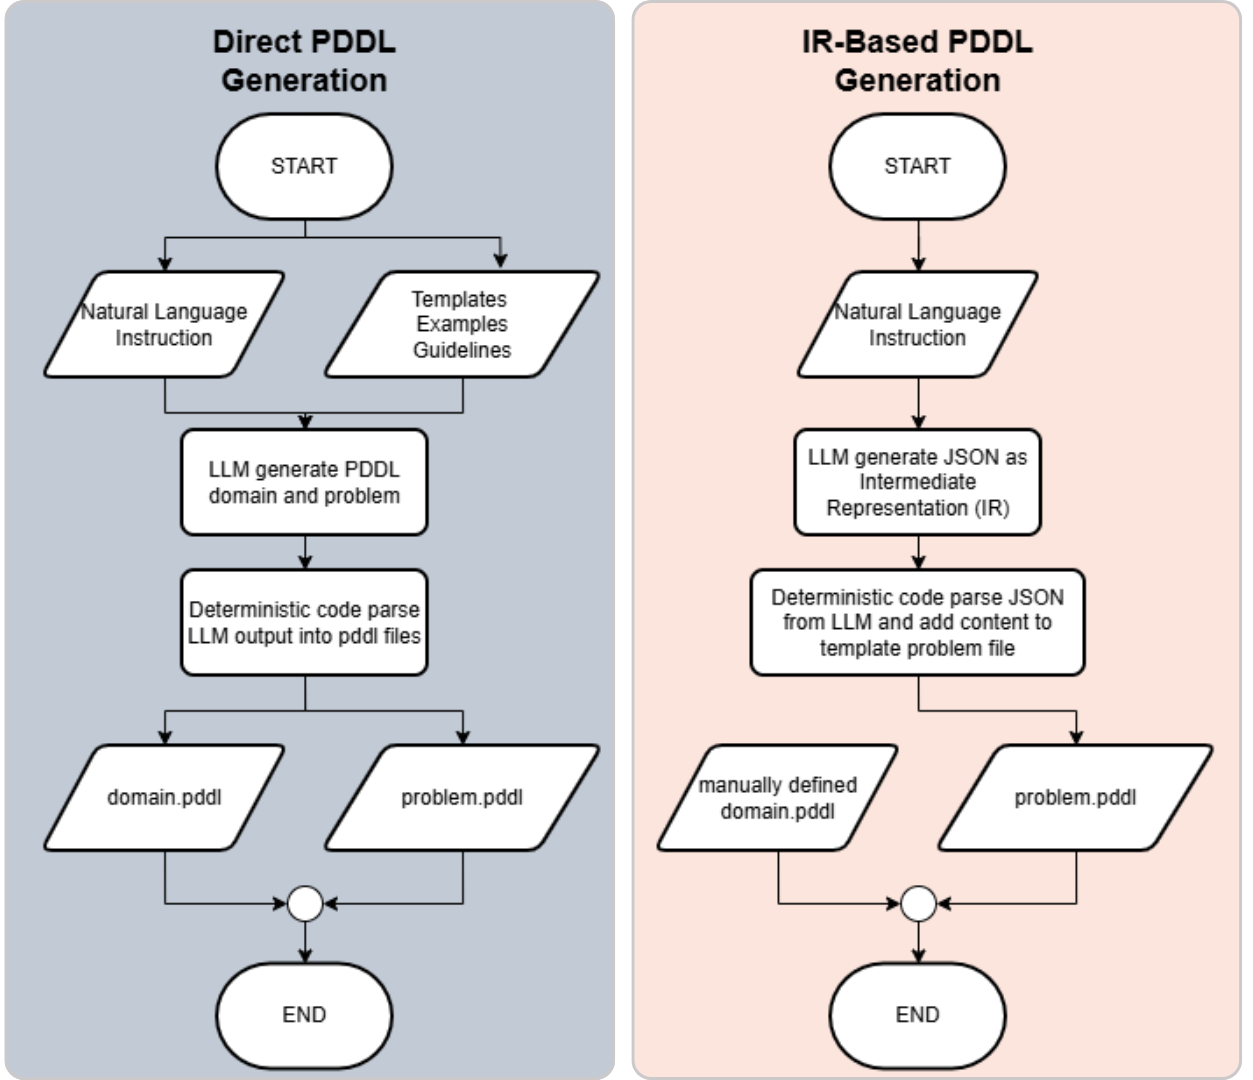
\includegraphics[width=\linewidth]{images/pddl_generation.png}
    \caption{Comparison of direct PDDL generation and the proposed IR-based pipeline}
    \label{fig:pddl-pipeline}
\end{figure}

\section{Experiments and Results}
\label{sec:experimental-setup}


We evaluate this approach on Blocksworld \cite{slaney2001blocks}. Each task includes an initial state (image) and a goal (natural language). The model must generate a valid PDDL problem that supports correct symbolic planning. Initial-state images come from BIRD~\cite{bird}. Because the LLM operates on textual input, a vision-language model (VLM) first converts each image into a textual state description, which is concatenated with the goal instruction. Each generated problem is solved with Fast Downward \cite{helmert2006fast} using a fixed domain file. We compare two approaches for PDDL generation:

\begin{itemize}
    \item \textbf{Direct Generation:} The LLM directly generates the full PDDL problem description from the input.
    \item \textbf{IR-based Generation:} The LLM first produces a structured intermediate representation, which is then deterministically converted into a PDDL problem file.
\end{itemize}


We evaluate four dimensions: correctness, validity, efficiency, and symbolic accuracy. \textit{Planning Success Rate} is a binary indicator of whether the generated PDDL yields a valid plan matching the ground-truth action sequence. \textit{Syntax Validity} is a binary indicator of whether Fast Downward can parse the generated PDDL without syntax errors. \textit{Efficiency}
Efficiency is measured by token usage and runtime. Token usage is estimated from input and output lengths, and elapsed time captures end-to-end latency. \textit{Symbolic Accuracy} is measured with the balanced F-score $F_{pd1}$, following prior work~\cite{planowl}. It captures overlap between generated and ground-truth objects, initial predicates, and goal predicates $F_{pd1} = \frac{2 \cdot P \cdot R}{P + R}$, where precision $P$ is the fraction of correct generated symbols and recall $R$ is the fraction of ground-truth symbols recovered. $F_{pd1} = 1.0$ indicates exact symbolic correspondence.

\subsection{Results}
\label{sec:results}



\begin{table*}[h]
\centering
\caption{Comparison between direct PDDL generation and IR-based (JSON) generation.}
\label{tab:main-results}
\begin{tabular}{lcccccc}
\toprule
\textbf{Approach} & \textbf{Plan Found (\%)} & \textbf{Syntax Valid (\%)} & \textbf{In. Tokens (mean)} & \textbf{Out. Tokens (mean)} & \textbf{Time (mean s)} \\
\midrule
Direct & 45.2 & 93.5 & 689.70 & 411.46 & 54.97 \\
IR & 65.8 & 97.1 & 624.89 & 51.23 & 54.30 \\
\bottomrule
\end{tabular}
\end{table*}


Table~\ref{tab:main-results} summarizes the performance of both approaches across planning success, syntactic validity, efficiency, and runtime metrics. IR-based generation improves planning success (65.8\% vs. 45.2\%) and syntax validity (97.1\% vs. 93.5\%) over direct generation. It also uses fewer input tokens (624.89 vs. 689.70) and far fewer output tokens (51.23 vs. 411.46), with comparable runtime. Table~\ref{tab:f1-results} reports the symbolic accuracy metrics based on precision, recall, and F1 score.

\begin{table}[h]
\centering
\caption{Symbolic accuracy comparison using $F_{pd1}$.}
\label{tab:f1-results}
\begin{tabular}{lccc}
\toprule
\textbf{Approach} & \textbf{Precision} & \textbf{Recall} & \textbf{F1} \\
\midrule
Direct  & 0.3730 & 0.3837 & 0.3756 \\
IR & 0.5784 & 0.5765 & 0.5732 \\
\bottomrule
\end{tabular}
\end{table}

IR-based generation yields higher precision, recall, and F1 than direct generation, improving macro F1 from 0.3756 to 0.5732.

\section{Discussion}
\label{sec:discussion}

The results show that introducing a structured intermediate representation improves the reliability of PDDL generation, as evidenced by higher syntactic validity and planning success rates. By constraining the output space, the IR-based approach reduces formatting errors and increases the likelihood of producing usable planning problems.

Improvements in symbolic accuracy further indicate that the intermediate representation helps the model better capture the structure of the task. Separating high-level specification from low-level syntax allows the model to focus on semantically meaningful elements, while deterministic conversion ensures correctness of the final PDDL output, reducing error propagation.

The reduction in token usage suggests that structured generation also improves efficiency, as the model no longer needs to produce verbose formal syntax or rely on extensive prompting. Execution time remains comparable between approaches, indicating that the primary benefit lies in output quality rather than speed.

More broadly, these results suggest that structured intermediate representations are an effective mechanism for improving LLM reliability when generating formal languages. This approach may extend to other domains requiring strict syntax and logical consistency, such as code generation and formal verification.

A limitation of this work is that the intermediate representation is manually designed, requiring domain knowledge. Additionally, evaluation is limited to the Blocksworld domain, and further validation in more complex settings is needed to assess generalization.

\section{Conclusion}
\label{sec:conclusion}

Dynamically generating plans given unforeseen world states is a critical task in robotics. 
The presented approach offers a simple but effective method to leverage the generative capabilities of LLMs to tackle the plan generation problem, addressing the limitations of LLM generation on precise syntax and semantics by leveraging structured output as an intermediate representation that can then be deterministically translated by other means. This approach broadens the use of generative AI for robotic applications. 


%%
%% The acknowledgments section is defined using the "acks" environment
%% (and NOT an unnumbered section). This ensures the proper
%% identification of the section in the article metadata, and the
%% consistent spelling of the heading.
\begin{acks}
The authors would like to thank the Robotics \& AI committee at the International School of Engineering, Faculty of Engineering, Chulalongkorn University, for financially supporting this project.
\end{acks}

%%
%% The next two lines define the bibliography style to be used, and
%% the bibliography file.
\bibliographystyle{ACM-Reference-Format}
\bibliography{refs-main}


%%
%% If your work has an appendix, this is the place to put it.


\end{document}
\endinput
%%
%% End of file `sample-acmlarge.tex'.
